\documentclass[compress]{beamer}

\usepackage[nofonts]{ctex}
\setCJKmainfont[ItalicFont={Kaiti SC}]{Kaiti SC}%
%\setCJKmainfont[ItalicFont={AR PL KaitiM GB}]{AR PL KaitiM GB}%
%\setCJKsansfont{WenQuanYi Zen Hei}% 文泉驿的黑体

\mode<beamer>
{
     \useinnertheme{rectangles}
     %\useoutertheme{infolines}
     \useoutertheme{split}
     \usecolortheme{rose}
     \usecolortheme{seahorse}

     \setbeamertemplate{navigation symbols}{}%remove navigation symbols

     \expandafter\def\expandafter\insertshorttitle\expandafter{%
     \insertshorttitle\hfill%
     \insertframenumber\,/\,\inserttotalframenumber}
     %\raisebox{-1ex}{
\includegraphics[width=3ex]{Overlays/logo.pdf}}}
}

%\defbeamertemplate*{footline}{mytheme}
%{
%  \leavevmode%
%  \hbox{%
%  \begin{beamercolorbox}[wd=.5\paperwidth,ht=2.25ex,dp=1ex,center]{author in head/foot}%
%    \usebeamerfont{author in head/foot}\insertshortauthor~~%
%    \raisebox{-1ex}{
\includegraphics[width=3ex]{Overlays/logo.pdf}}%
%  \end{beamercolorbox}%
%  \begin{beamercolorbox}[wd=.5\paperwidth,ht=2.25ex,dp=1ex,right]{title in head/foot}%
%    \usebeamerfont{title in head/foot}\insertshorttitle{}\hspace*{2em}
%    \insertframenumber{} / \inserttotalframenumber\hspace*{2ex} 
%  \end{beamercolorbox}}%
%  \vskip0pt%
%}
%\usebeamertemplate{mytheme}

%\setbeamercovered{transparent}

\mode<handout>
{
	\usetheme{default}
	\usepackage{pgfpages}
	\pgfpagesuselayout{4 on 1}[a4paper,landscape,border shrink=5mm]
}


\usepackage[utf8]{inputenc}
\usepackage{amsmath,latexsym,amssymb,amsfonts,amsbsy}
\usepackage{graphicx}
\usepackage{array}
\usepackage{hyperref}
\usepackage{fancyvrb}
\usepackage{listings}
\usepackage{textpos}
\usepackage{ulem}
\usepackage{comment}
\usepackage{tikz}
\usetikzlibrary{calc,arrows.meta, graphs, trees, shapes, positioning, decorations.markings, intersections, decorations.text}
\usepackage{tikz-uml}

\newcommand{\romannumber}[1]{{\textrm{\uppercase\expandafter{\romannumeral
#1}}}}

\setbeamercolor{dblue}{fg=white,bg=gray!70!blue} % for beamercolorbox
 \newenvironment{pblock}{\begin{beamercolorbox}[rounded=true,
          shadow=false]{dblue}}{\end{beamercolorbox}}
 \newenvironment{bblock}{\begin{beamercolorbox}[rounded=true,
          shadow=false]{fg=black, bg=white}}{\end{beamercolorbox}}

\graphicspath{{figure/}}

\lstset{
	basicstyle=\footnotesize\ttfamily, % print whole listing footnotesize
	keywordstyle=\footnotesize\color{black}\ttfamily\bfseries, 
	identifierstyle=\footnotesize\color{blue}\ttfamily, 
	commentstyle=\footnotesize\itshape\ttfamily, 
	stringstyle=\footnotesize\ttfamily,
	frame=single, 
	numbers=left, numberstyle=\tiny,
	stepnumber=1, numbersep=10pt,
	showtabs=false, tabsize=4,
	showstringspaces=false,
	breaklines=true, breakatwhitespace=true,
	language=[ISO]C++
}   

 
%%%%%%%%%%%%%%%%%%%%%%%%%%%%%%%%%%%%%%%%%%%%%%%%%%%%%%%%%%%%%%%%%
%    body                                                       %
%%%%%%%%%%%%%%%%%%%%%%%%%%%%%%%%%%%%%%%%%%%%%%%%%%%%%%%%%%%%%%%%%


\begin{document}

\AtBeginSubsection[]
{ 
    \begin{frame}<beamer> 
		\frametitle{内容提要} 
		\tableofcontents[currentsection,currentsubsection,
        subsectionstyle=show/shaded/hide] 
	\end{frame} 
} 

					
\title{第八章 ~~ 面向对象的系统设计\MakeUppercase{\romannumeral 2}}

\author[面向对象的分析与设计]
{曹东刚\\\href{mailto:caodg@pku.edu.cn}{caodg@pku.edu.cn}}

\institute[北京大学]{北京大学信息学院研究生课程 - 面向对象的分析与设计 \\
\href{http://c.pku.edu.cn/}{http://c.pku.edu.cn/}}

\date{}

\titlegraphic{
\includegraphics[height=0.10\textwidth]{Overlays/logo.pdf}}

\begin{frame}[plain]
	\titlepage
\end{frame}

\setcounter{framenumber}{0}

\section{控制驱动部分的设计}

\subsection[背景]{背景及相关技术介绍}

\begin{frame}
  \frametitle{什么是控制驱动部分}
  \begin{block}{控制驱动部分}
    是OOD模型的外围组成部分之一,由系统中全体\uline{主动类}构成。这些
    主动类描述了整个系统中所有的\uline{主动对象},每个主动对象是系统中一
    个\uline{控制流}的驱动者 
  \end{block}

  控制流(control flow):\uline{进程}(process)和\uline{线程}(thread)的总称 \\

  有多个控制流并发执行的系统称作\uline{并发系统}(多任务系统)

\end{frame}

\begin{frame}
  \frametitle{为什么需要控制驱动部分}
  \begin{itemize}
    \item 并发行为是现实中固有的
      \begin{itemize}
        \item 外围设备与主机并发工作的系统
        \item 有多个窗口进行人机交互的系统
        \item 多用户系统
        \item 多个子系统并发工作的系统
        \item 单处理机上的多任务系统
        \item 多处理机系统
      \end{itemize}

    \item 多任务的设置
      \begin{itemize}
        \item 描述问题域固有的并发行为
        \item 表达实现所需的设计决策
      \end{itemize}

    \item 隔离硬件、操作系统、网络的变化对整个系统的影响
  \end{itemize}
\end{frame}


\begin{frame}
  \frametitle{由系统总体方案决定的实现条件}
  \begin{itemize}
    \item 计算机硬件:性能、容量和CPU数目
    \item 操作系统:对并发和通讯的支持
    \item 网络方案:网络软硬件设施、网络拓扑结构、通讯速率、网络协议等
    \item 软件体系结构
    \item 编程语言:对进程和线程的描述能力
    \item 其它软件:如数据管理系统、界面支持系统、构件库等
  ——对共享和并发访问的支持
  \end{itemize}
\end{frame}

\begin{frame}
  \frametitle{软件体系结构}
  \begin{block}{软件体系结构}
    描述了构成系统的元素、这些元素之间的相互作用、指导其组合的
  模式以及对这些模式的约束
\end{block}
几种典型的软件体系结构风格
\begin{itemize}
  \item 管道与过滤器风格(pipe and filter style)
  \item 面向对象风格(object-oriented style)
  \item 层次风格(layered style)
  \item 黑板风格(blackboard style)
  \item 进程控制风格(process control style)
  \item 客户-服务器风格(client-server style) 
\end{itemize}

\end{frame}

\begin{frame}
  \frametitle{分布式系统的体系结构风格}
  \begin{itemize}
    \item 主机+仿真终端体系结构
    \item 文件共享体系结构
    \item 客户-服务器体系结构
      \begin{itemize}
        \item 二层客户-服务器体系结构
        \item 三层客户-服务器体系结构
        \item 对等式客户-服务器体系结构
        \item 瘦客户-服务器体系结构
        \item 胖客户-服务器体系结构
      \end{itemize}
    \item 浏览器-服务器体系结构
  \end{itemize}

\end{frame}

\begin{frame}
  \frametitle{系统的并发性}
  \only<1> {
    进程(process)概念出现之前,并发程序设计困难重重,
    主要原因:
    \begin{itemize}
      \item 并发行为彼此交织,理不出头绪
      \item 与时间有关的错误不可重现
    \end{itemize}

    \uline{进程}概念的提出使这个问题得到根本解决
  }

  \only<2> {
    进程的全称是\uline{顺序进程}(sequential process),其基本思想是把并发程序分
    解成一些顺序执行的进程,使得:

    \begin{itemize}
      \item 每个进程内部不再包含并发行为 \\
    \quad 所以叫做顺序进程,其设计避免了并发问题
      \item 多个进程之间是并发(异步)执行的 \\
    \quad 所以能够构成并发程序
    \end{itemize}
  }
\end{frame}

\begin{frame}
  \frametitle{进程与线程}
  由于并行计算的需要,要求人为地在\uline{顺序程序内部}定义和识别可
  \uline{并发执行}的单位
  ,线程的概念就诞生了 \\[2ex]

  \textcolor{blue}{线程与进程的区别}:

  \begin{itemize}
    \item 进程既是处理机分配单位,也是存储空间、设备等资源的分配单位(重量级的控
  制流)

\item 线程只是处理机分配单位(轻量级的控制流) 

\item 一个进程可以包含多个线程,也可以是单线程的
  \end{itemize}
\end{frame}

\begin{frame}
  \frametitle{应用系统的并发性}
  \only<1> {
  \textcolor{blue}{ 从网络、硬件平台的角度看}:
  \begin{itemize}
    \item 分布在不同计算机上的进程之间的并发
    \item 在多CPU的计算机上运行的进程或线程之间的并发
    \item 在一个CPU上运行的多个进程或线程之间的并发
  \end{itemize}
}

\only<2> {
  \textcolor{blue}{从应用系统的需求看}:
  \begin{itemize}
    \item 需要跨地域进行业务处理的系统
    \item 需要同时使用多台计算机或多个CPU进行处理的系统
    \item 需要同时供多个用户或操作者使用的系统
    \item 需要在同一时间执行多项功能的系统
    \item 需要与系统外部多个参与者同时进行交互的系统
  \end{itemize}
}
\end{frame}

\begin{frame}
  \frametitle{处理应用系统并发的例子}

  \label{app:satallite}
  \only<1> {
    \textbf{问题描述:} \\[2ex]
    某单位想开发一个卫星遥感信息处理系统,要求是:实时把通过地面接收设备
    传来的卫星遥感图片信息\uline{输入系统},经过必要的\uline{数据处理},
    及时将图片\uline{显示在屏幕上}。
  }

  \only<2> {
  \centering\begin{figure}
  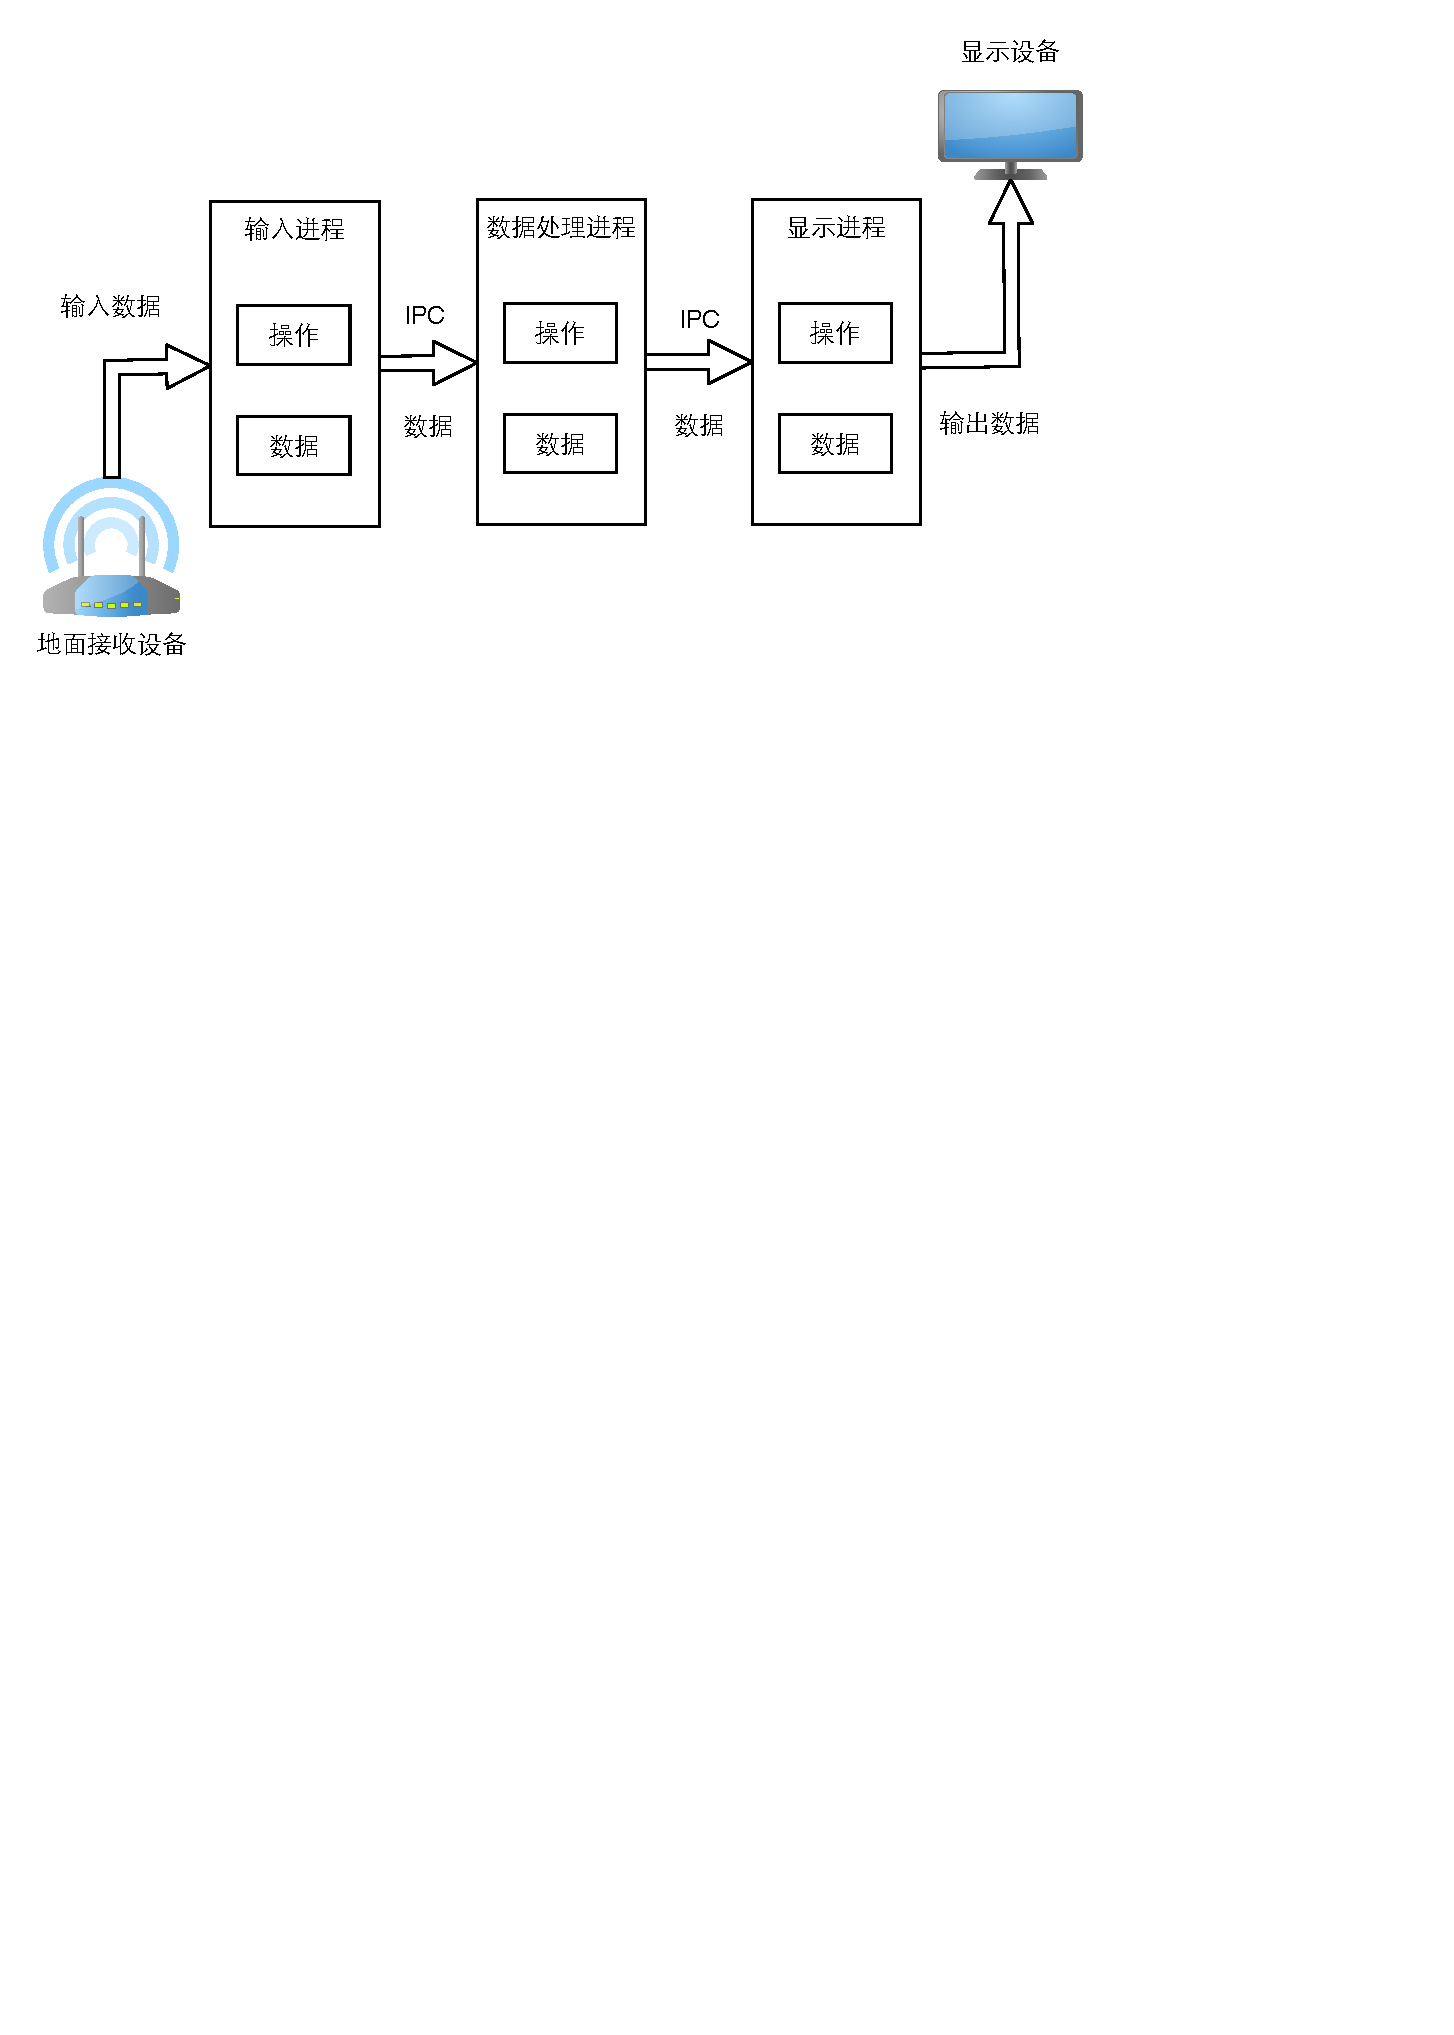
\includegraphics[width=0.9\hsize]{yaogan-processes.pdf}

  用多进程实现的遥感信息处理系统
  \end{figure}
  }

  \only<3> {
    \textbf{新的需求:} \\[2ex]
    针对前页\ref{app:satallite}例子中多进程共享数据速度慢的问题,希望改
    变设计,采用\uline{多线程技术}实现并发,避免控制流之间传送大量数据。
  }
  \only<4> {
  \centering\begin{figure}
  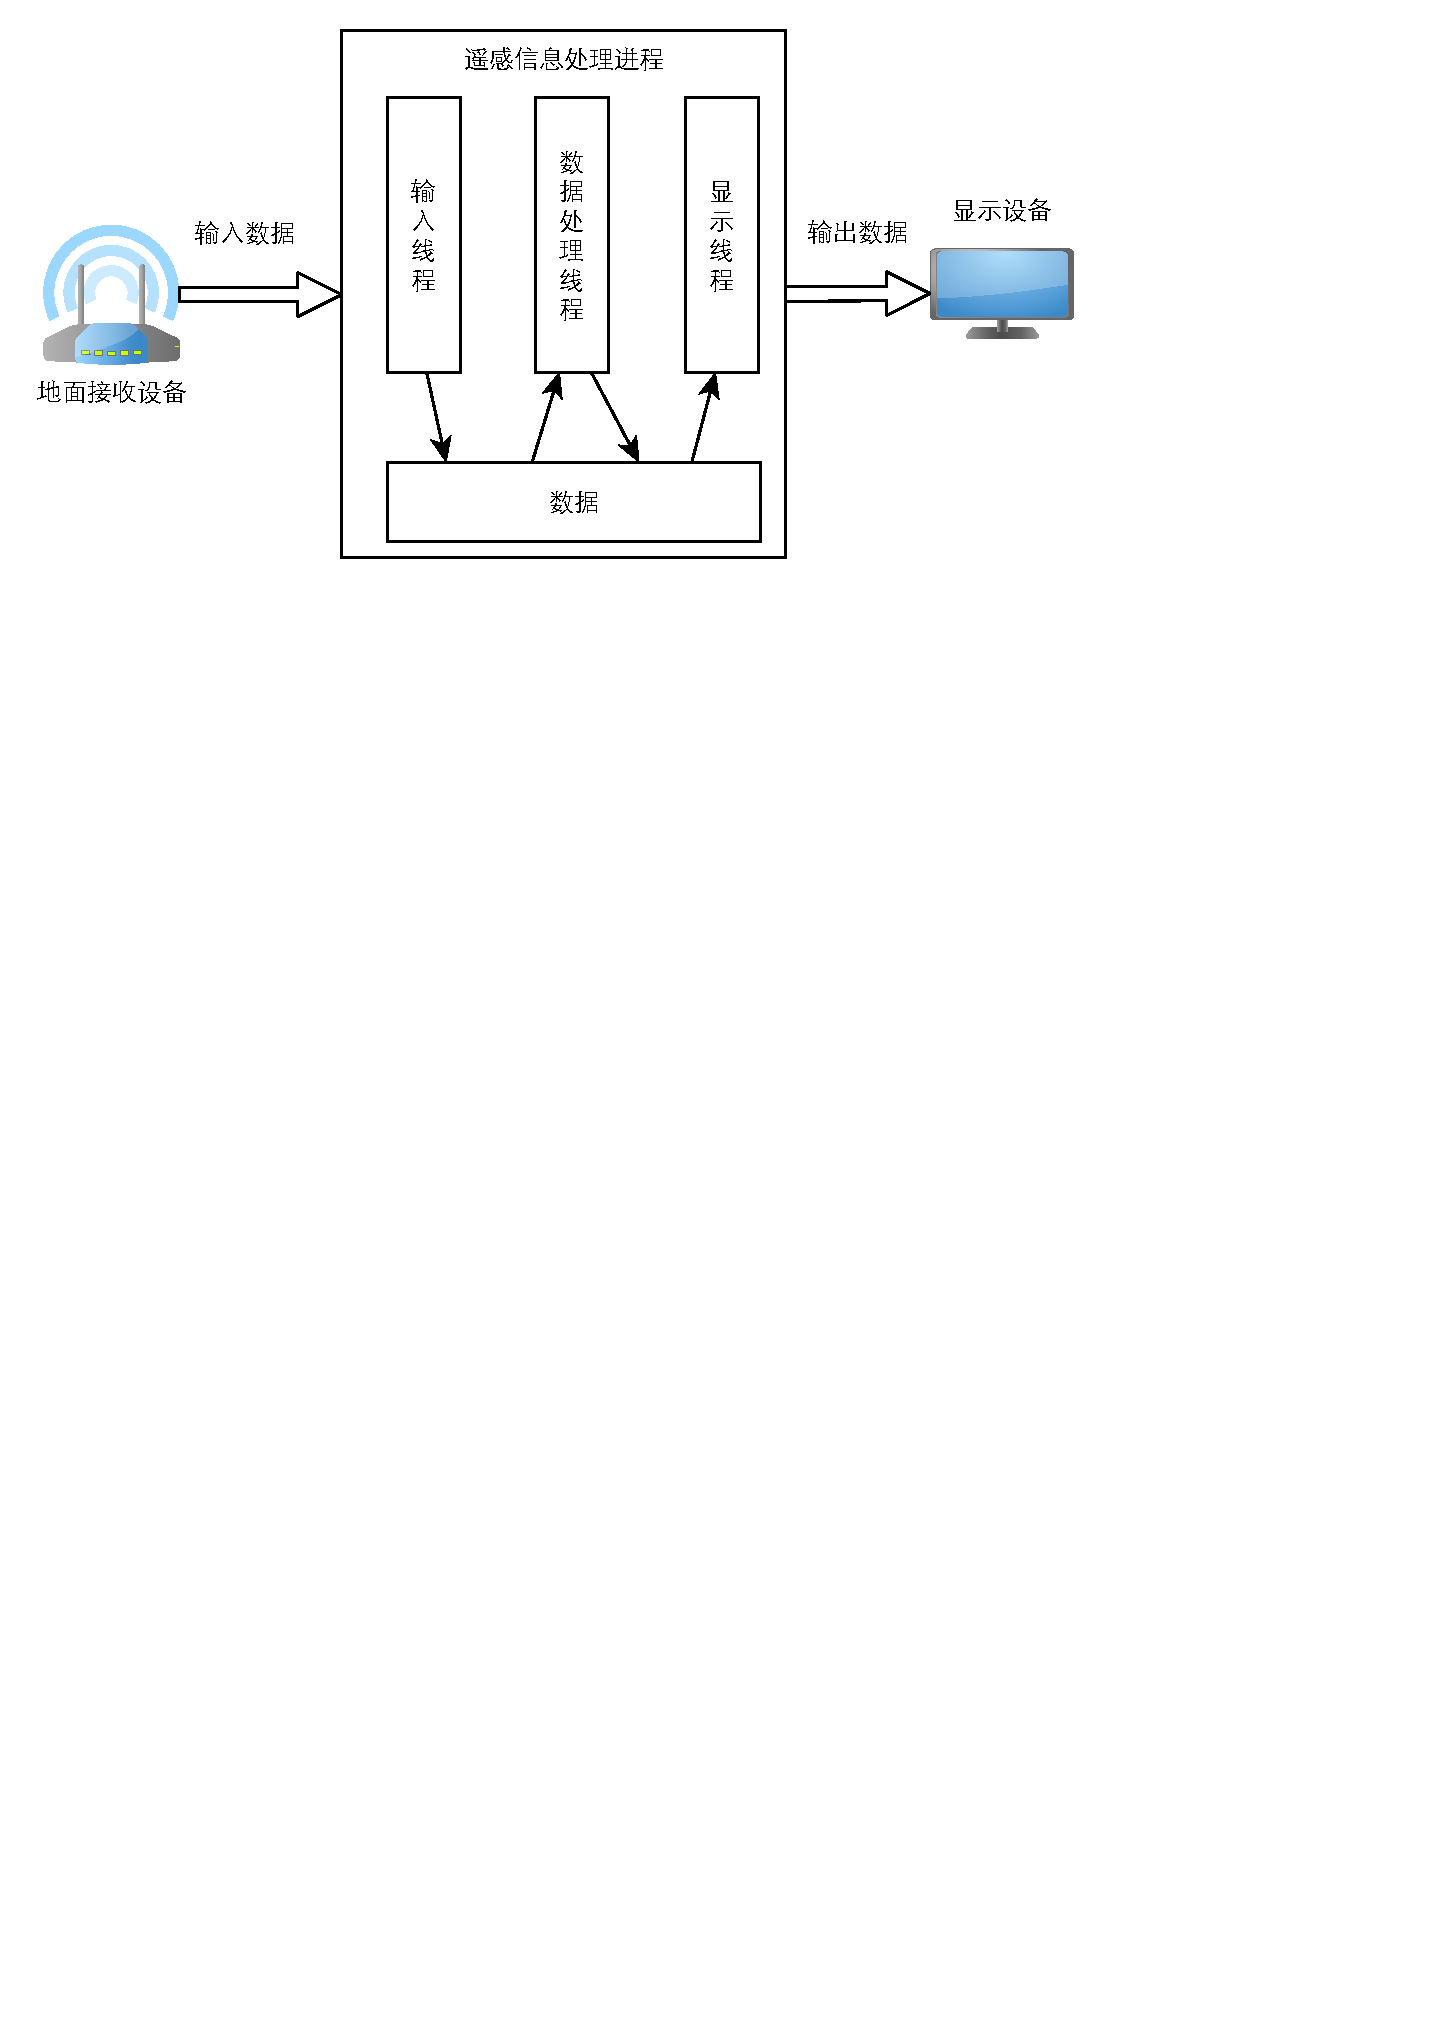
\includegraphics[width=0.9\hsize]{yaogan-threads.pdf}

  用多线程实现的遥感信息处理系统
  \end{figure}
  }

  \only<5> {
    \textbf{拓展业务:} \\[2ex]
    考虑面向不同应用的遥感信息处理系统,不仅需要把图片信息实时显示出来,
    而且需进行\uline{更多处理},如面向地理信息系统的特征信息提取等。
  }
  \only<6> {
  \centering\begin{figure}
  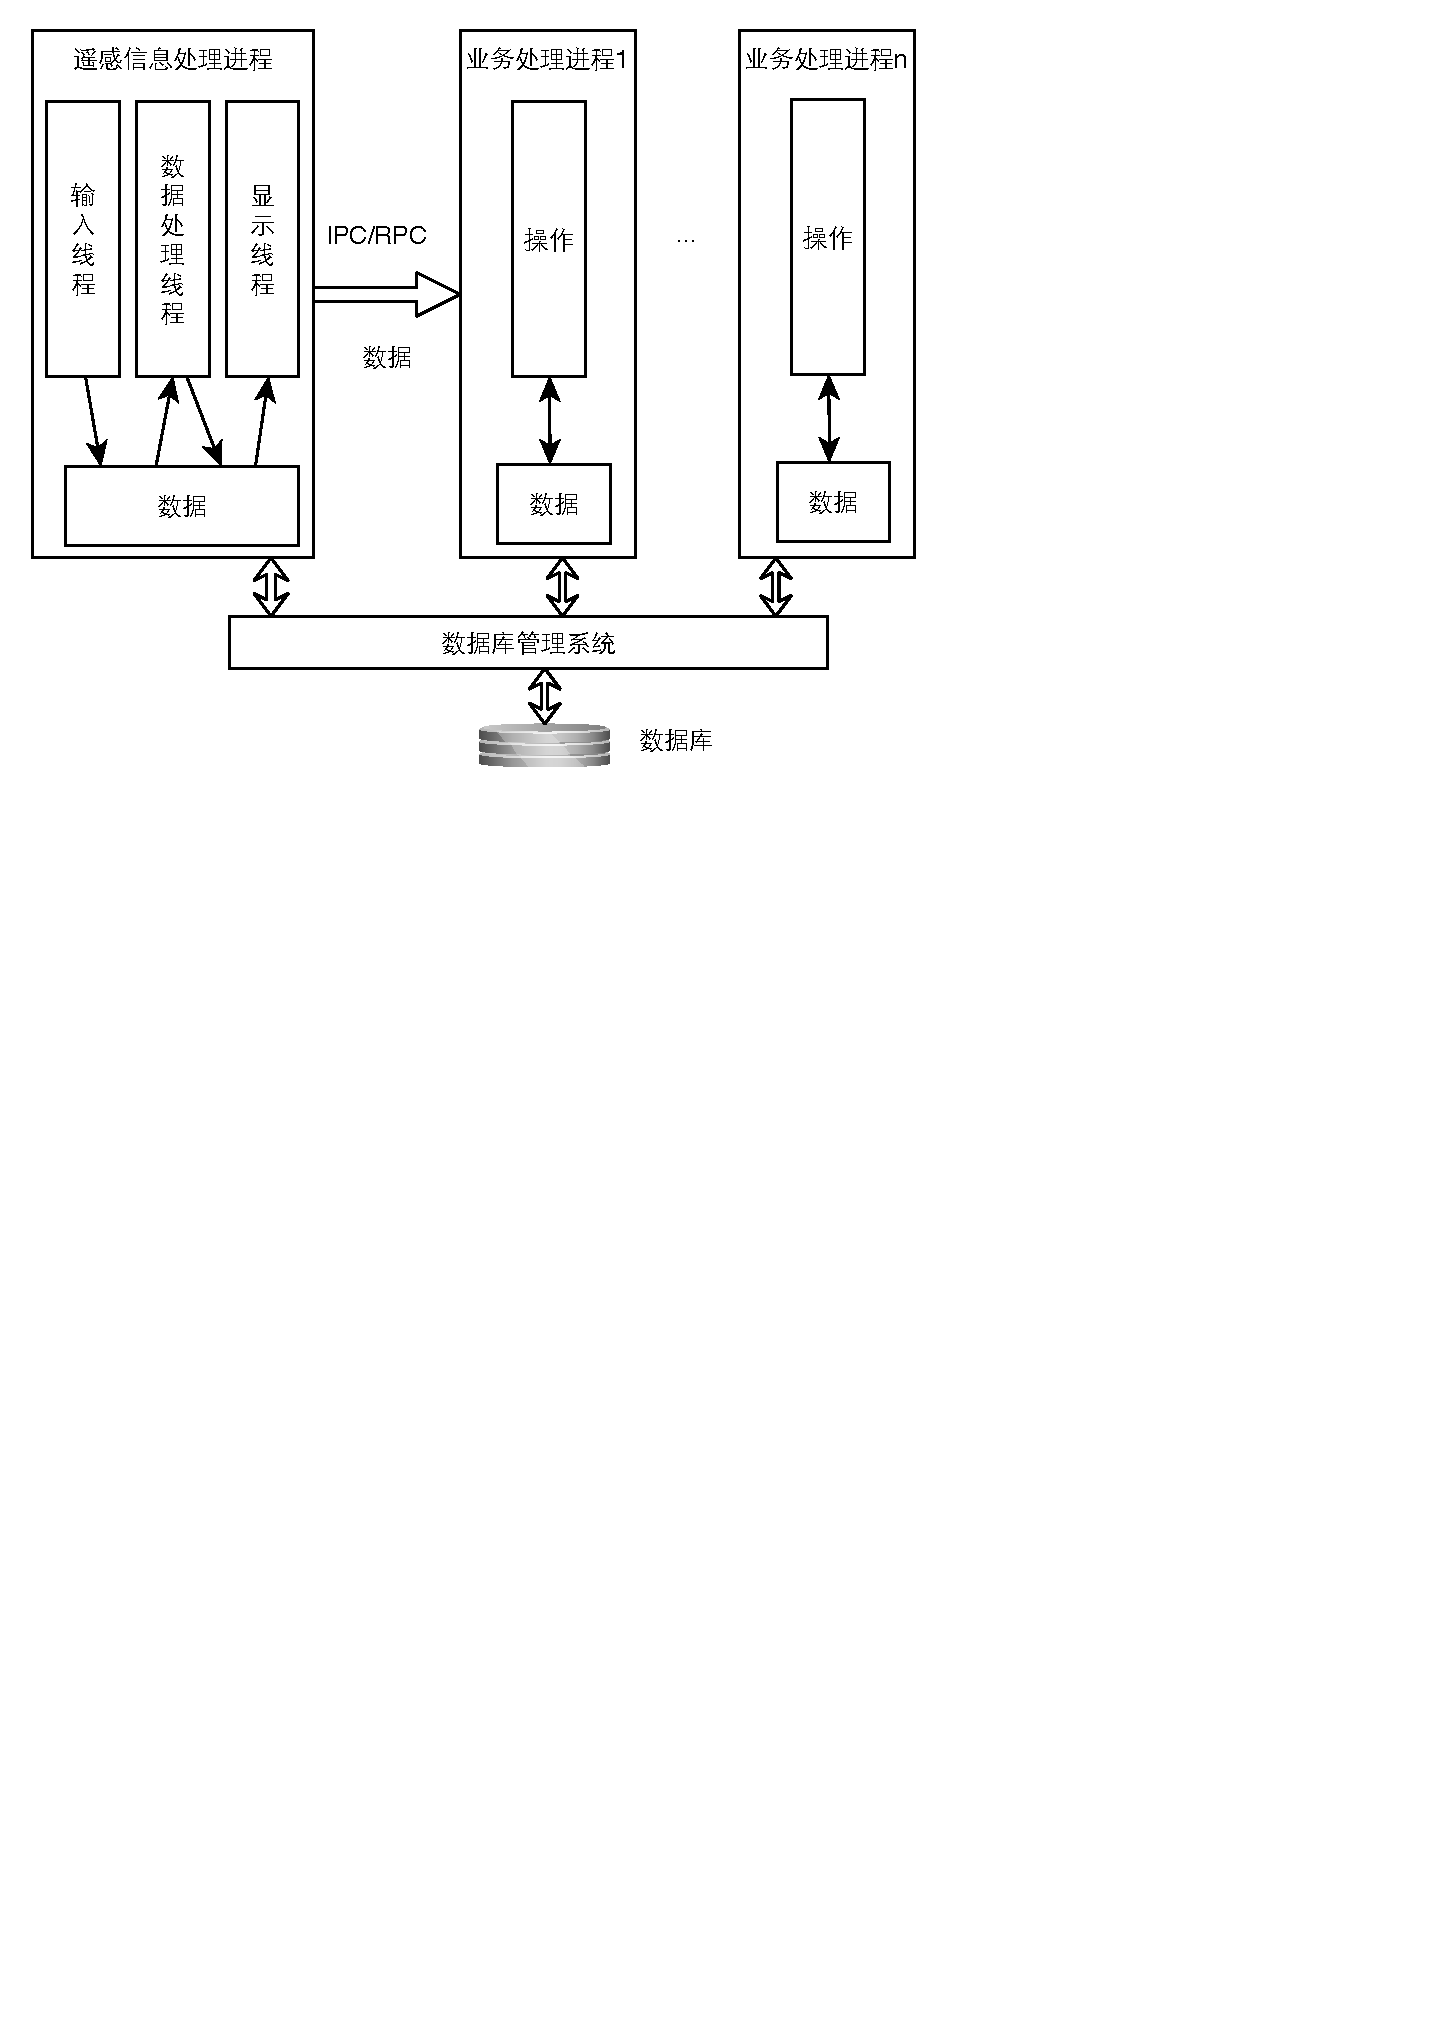
\includegraphics[width=0.8\hsize]{yaogan-mix.pdf}

  同时采用多线程和多进程的多应用遥感信息处理系统
  \end{figure}
  }
\end{frame}

\begin{frame}
  \frametitle{讨论:进程 vs 线程}
  \fbox{
    \parbox{0.8\hsize} {
    \textbf{进程}:重量,分布内存 \\
    \textbf{线程}:轻量,共享内存
    }
  } \\[2ex]

  \begin{itemize}
    \item 数据访问的成本和效率?
    \item 创建、销毁、切换的代价?
    \item 健壮性?
    \item 易于程序员编写并发程序?
  \end{itemize}
\end{frame}

\subsection[如何设计]{如何设计控制驱动部分}

\begin{frame}
  \frametitle{选择软件体系结构风格}

  \begin{itemize}
    \item 二层客户--服务器体系结构 \\
    (数据)服务器--客户机
    \item 三层客户--服务器体系结构 \\
    数据服务器--应用服务器--客户机 
  \end{itemize}
\end{frame}

\begin{frame}
  \frametitle{确定系统分布方案}

  \only<1> {
  \fbox{
    \parbox{0.8\hsize}{
      考虑分布方案\uline{之前}:\uline{暂时}将系统看作\uline{集中式}的 \\
      确定分布方案\uline{之后}:将对象分布到各个处理机上, \\
以\textcolor{blue}{每台处理机上的类作为一个包}
   }
 } \\[2ex]

  \begin{tikzpicture}
    \tikzumlset{fill package=white}
    \node [rectangle, draw, align=center,  
      minimum width=1.5cm, minimum height=3cm] {集中式 \\类图} ;
    \draw [->, line width=2pt, >=stealth] (1.2, 0) -- ( 2.2, 0) ; 
    \draw [->, line width=2pt, >=stealth] (1.2, 0.5) -- ( 2.2, 1) ; 
    \draw [->, line width=2pt, >=stealth] (1.2, -0.5) -- ( 2.2, -1) ; 
    \begin{umlpackage}[x=3.5, y=1.5]{A}
    \end{umlpackage}
    \begin{umlpackage}[x=3.5, y=-1.5]{B}
    \end{umlpackage}
    \begin{umlpackage}[x=6.5]{C}
    \end{umlpackage}
    \node[right=0.4 of A.north west, yshift=+0.3cm] { \footnotesize 部署于主机a} ;
    \node[right=0.4 of B.north west, yshift=+0.3cm] { \footnotesize 部署于主机b} ;
    \node[right=0.4 of C.north west, yshift=+0.3cm] { \footnotesize 部署于主机c} ;
  \end{tikzpicture}
  }

  \only<2> {
    系统分布包括\textcolor{blue}{功能分布}和\textcolor{blue}{数据分布},
    在面向对象的系统中都体现于\uline{对象分布} \\[2ex]

    \alert{原则}:\uline{减少远程传输,便于管理} \\[2ex]

    \alert{决定对象分布}:
    \begin{itemize}
      \item 软件体系结构
      \item 系统功能在哪些结点提供
      \item 数据在哪些结点长期存储管理,在哪些结点临时使用
      \item 参照用况,把合作紧密的对象尽可能分布在同一结点
      \item 追踪消息,把一个控制流经历的对象分布在同一结点
    \end{itemize}

  }

  \only<3> {
    类的分布:\uline{根据对象分布的需要} \\

    分布在每个结点上的对象,都需要相应的类来创建

    \begin{itemize}
    \item [策略1] 如果一个类只需要在一个结点上创建对象实例:\\
        {把这个类分布在该结点上}

      \item [策略2] 如果一个类需要在多个结点上创建对象实例: \\
    把这个类分布到每个需要创建其实例的结点上, \\
    其中一个作为正本,其他作为副本
    \end{itemize}
  }

  \only<4> {
    \centering\begin{figure}
    \scalebox{0.8} {
    \begin{tikzpicture}
      \tikzumlset{fill class=white}
      \umlemptyclass{A}
      \umlemptyclass[x=-1.5, y=-3]{C}
      \umlemptyclass[x=1.5, y=-3, fill=yellow!20]{D}
      \umlemptyclass[x=1.5, y=-6]{G}
      \umlemptyclass[x=-4.5, y=-3]{B}
      \umlemptyclass[x=-4.5, y=-6]{E}
      \umlemptyclass[x=-1.5, y=-6]{F}

      \umlemptyclass[x=5]{H}
      \umlemptyclass[x=5, y=-3]{I}
      \umlemptyclass[x=5, y=-6]{J}

      \umlinherit[geometry=|-|]{C}{A}
      \umlinherit[geometry=|-|]{D}{A}
      \umlinherit{G}{D}
      \umlinherit{I}{H}
      \umluniassoc{B}{C}
      \umlaggreg{B}{E}
      \umlassoc[mult1=1, mult2=*]{G}{F}
      \umlassoc[mult1=1, mult2=*]{I}{J}
      \umldep[stereo=call]{I}{D}
    \end{tikzpicture}
    }

    例:一个集中式类图
  \end{figure}
  }

  \only<5> {
    \centering\begin{figure}
    \scalebox{0.7} {
    \begin{tikzpicture}
      \tikzumlset{fill class=white, fill package=white}
      \begin{umlpackage}{Server Package}
      \umlemptyclass{A}
      \umlemptyclass[x=-1.5, y=-3]{C}
      \umlemptyclass[x=1.5, y=-3, fill=yellow!20]{D}
      \umlemptyclass[x=1.5, y=-6]{G}
      \umlemptyclass[x=-4.5, y=-3]{B}
      \umlemptyclass[x=-4.5, y=-6]{E}
      \umlemptyclass[x=-1.5, y=-6]{F}

      \umlinherit[geometry=|-|]{C}{A}
      \umlinherit[geometry=|-|]{D}{A}
      \umlinherit{G}{D}
      \umluniassoc{B}{C}
      \umlaggreg{B}{E}
      \umlassoc[mult1=1, mult2=*]{G}{F}
    \end{umlpackage}
    \end{tikzpicture}
    }

    例:服务器包
  \end{figure}

  }

  \only<6> {
    \centering\begin{figure}
    \scalebox{0.7} {
    \begin{tikzpicture}
      \tikzumlset{fill class=white, fill package=white}
      \begin{umlpackage}{Client Package}
        \umlemptyclass[type=副本]{A}
      \umlemptyclass[y=-3, draw=red, text=red, type=副本]{D}

      \umlemptyclass[x=4]{H}
      \umlemptyclass[x=4, y=-3]{I}
      \umlemptyclass[x=4, y=-6]{J}

      \umlinherit{D}{A}
      \umlinherit{I}{H}
      \umlassoc[mult1=1, mult2=*]{I}{J}
      \umldep[stereo=call]{I}{D}
    \end{umlpackage}
    \end{tikzpicture}
    }

    例:客户机包 (第一种策略)
  \end{figure}

  }

  \only<7> {
    \centering\begin{figure}
    \scalebox{0.7} {
    \begin{tikzpicture}
      \tikzumlset{fill class=white, fill package=white}
      \begin{umlpackage}{Client Package}
      \umlemptyclass[y=-3, draw=red, text=red, type=副本]{D}

      \umlemptyclass[x=4]{H}
      \umlemptyclass[x=4, y=-3]{I}
      \umlemptyclass[x=4, y=-6]{J}

      \umlinherit{I}{H}
      \umlassoc[mult1=1, mult2=*]{I}{J}
      \umldep[stereo=call]{I}{D}
    \end{umlpackage}
    \end{tikzpicture}
    }

    例:客户机包 (第二种策略)
  \end{figure}

  }

\end{frame}

\begin{frame}
  \frametitle{识别控制流}
  \only<1> {
  \begin{enumerate}
    \item 以结点为单位识别控制流
      \begin{itemize}
        \item 不同结点上程序的并发问题已经解决
        \item 考虑在每个结点上运行的程序还需要如何并发 
      \end{itemize}
    \item 从用户需求出发认识控制流
      \begin{itemize}
        \item 有哪些任务必须在同一台计算机上并发执行 
      \end{itemize}
    \item 从用况认识控制流  关注描述如下三类功能的用况
      \begin{itemize}
        \item 要求与其他功能同时执行的功能
        \item 用户随时要求执行的功能
        \item 处理系统异常事件功能
      \end{itemize}
  \end{enumerate}
  }

  \only<2> {
    \begin{enumerate}
    \setcounter{enumi}{3}
      \item 参照OOA模型中的主动对象
      \item 为改善性能而增设的控制流
        \begin{itemize}
          \item 高优先级任务
          \item 低优先级任务
          \item 紧急任务
        \end{itemize}
      \item 实现并行计算的控制流(线程/进程)
      \item 实现结点之间通讯的控制流(进程)
      \item 对其它控制流进行协调的控制流
    \end{enumerate}
  }

\end{frame}

\begin{frame}
  \frametitle{用主动对象表示控制流}
  \only<1> {
  \begin{block}{控制流}
    是主动对象中一个主动操作的一次执行。其间可能要调用其他对象的操作
  ,后者又可能调用另外一些对象的操作,这就是一个控制流的运行轨迹。 
\end{block}
\vspace*{2ex}
\begin{figure}
\begin{tikzpicture}
  \tikzumlset{fill class=white}
  \umlemptyclass[type=active]{Class A}
  \umlemptyclass[x=2.5, type=process]{Class B}
  \umlemptyclass[x=5, type=thread]{Class C}
  \umlemptyclass[x=7.5]{Class D}

  \draw (Class D.north west) -- ++(-0.1cm, 0) |- (Class D.south west) ;
  \draw (Class D.north east) -- ++(+0.1cm, 0) |- (Class D.south east) ;
\end{tikzpicture}

UML1和UML2中的主动类表示法
\end{figure}
  }

  \only<2> {
    \alert{问题}: \\
    \quad 一个主动类可以有多个主动操作和若干被动操作,UML的表示法如何显式地表示
    哪个(哪些)操作是主动操作? \\[2ex]
  }

  \only<3> {
    用\textcolor{blue}{关键词}表示主动操作 \\[3ex]
    \centering\begin{tikzpicture}
      \umlclass[type=active, fill=white]{Class Name}{}{
        \textcolor{blue}{<<process>> 操作名()} \\
        \quad \textcolor{blue}{<<thread>> 操作名()} \\
        \quad \textcolor{blue}{<<thread>> 操作名()} \\
        \textcolor{blue}{\ldots} \\
        操作名() \\
      \ldots
    }
    \end{tikzpicture}
  }

  \only<4> {
    \textcolor{blue}{显式}地表示由进程\uline{创建}线程 \\[2ex]

    \begin{tikzpicture}
      \tikzumlset{fill class=white}

      \umlclass[type=active] {A}{}{\textcolor{blue}{<<process>> P}}
      \umlclass[type=active, x=-3, y=-3] {B}{}
        {\textcolor{blue}{<<thread>> T1} }
      \umlclass[type=active, x=3, y=-3] {C}{}
        {\textcolor{blue}{<<thread>> T2} }

      \umldep[stereo=create, geometry=-|, pos stereo=1.6]{A}{B}
      \umldep[stereo=create, geometry=-|, pos stereo=1.6]{A}{C}
    \end{tikzpicture}
  }

\end{frame}

\begin{frame}
  \frametitle{主动对象在OOD模型中的位置}

\only<1> {
\begin{figure}
  \scalebox{0.8}{
    \begin{tikzpicture}
\renewcommand\baselinestretch{1.0}
\tikzstyle{Class}=[draw, rectangle, color=red, fill=yellow!20, align=center];
\tikzstyle{Depend}=[->, >=angle 60, color=red, dashed, thick];

%\draw [help lines, step=0.5cm] (0,0) grid (8,7) ;

\draw [very thick] (0,0) -- (8,0) -- (8,7) -- (0,7) -- (0,0) ;
\draw (0,0) -- (2.5,2.5) -- (2.5,7);
\draw (8,0) -- (5.5,2.5) -- (5.5,7);
\draw (2.5,2.5) -- (5.5,2.5) ;
\node [text width=1pt] at (1.0,5.5) {人机交互部分} ;
\node [text width=1pt] at (6.5,5.5) {数据接口部分} ;
\node at (4.0,0.5) {控制驱动部分} ;
\node at (4.0,6.5) {问题域部分} ;

\node [Class] (Seller) at (4.0,4.5) {营业员} ;
\node [Class] (SellerG) at (1.3,3.0) {营业员\\ 窗口} ;
\node [Class] (SellerP) at (4.0,1.7) {<<active>> \\ 营业员进程} ;

\draw [Depend] (SellerP) -- ( Seller) node [anchor=north west, yshift=-0.3cm] {<<call>>};
\draw [Depend] (Seller) -- ( SellerG) node [anchor=south west, xshift=0.7cm] {<<call>>};
\end{tikzpicture}
}

订单系统中营业员对象:无交叉方案
\end{figure}
}

\only<2> {
  \begin{figure}
    \scalebox{0.8}{
\begin{tikzpicture}
\renewcommand\baselinestretch{1.0}
\tikzstyle{Class}=[draw, rectangle, color=red, fill=yellow!20, align=center];
\tikzstyle{Depend}=[->, >=angle 60, color=red, dashed, thick];

%\draw [help lines, step=0.5cm] (0,0) grid (8,7) ;

\draw [very thick] (0,0) -- (8,0) -- (8,7) -- (0,7) -- (0,0) ;
\draw (0,0) -- (2.5,2.5) -- (2.5,7);
\draw (8,0) -- (5.5,2.5) -- (5.5,7);
\draw (2.5,2.5) -- (5.5,2.5) ;
\node [text width=1pt] at (1.0,5.5) {人机交互部分} ;
\node [text width=1pt] at (6.5,5.5) {数据接口部分} ;
\node at (4.0,0.5) {控制驱动部分} ;
\node at (4.0,6.5) {问题域部分} ;

\node [Class] (SellerG) at (1.3,3.0) {营业员\\ 窗口} ;
\node [Class] (SellerP) at (4.0,2.5) {<<process>> \\ 营业员} ;

\draw [Depend] (SellerP) -- ( SellerG) node [anchor=south west, xshift=0.7cm] {<<call>>};
\end{tikzpicture}
}

订单系统中营业员对象:问题域和控制驱动部分交叉
\end{figure}
}

\only<3> {
  \begin{figure}
    \scalebox{0.8}{
\begin{tikzpicture}
\renewcommand\baselinestretch{1.0}
\tikzstyle{Class}=[draw, rectangle, color=red, fill=yellow!20, align=center];
\tikzstyle{Depend}=[->, >=angle 60, color=red, dashed, thick];

%\draw [help lines, step=0.5cm] (0,0) grid (8,7) ;

\draw [very thick] (0,0) -- (8,0) -- (8,7) -- (0,7) -- (0,0) ;
\draw (0,0) -- (2.5,2.5) -- (2.5,7);
\draw (8,0) -- (5.5,2.5) -- (5.5,7);
\draw (2.5,2.5) -- (5.5,2.5) ;
\node [text width=1pt] at (1.0,5.5) {人机交互部分} ;
\node [text width=1pt] at (6.5,5.5) {数据接口部分} ;
\node at (4.0,0.5) {控制驱动部分} ;
\node at (4.0,6.5) {问题域部分} ;

\node [Class] (SellerG) at (2.5,5.0) {营业员\\ 窗口} ;
\node [Class] (SellerP) at (4.0,1.5) {<<process>> \\ 营业员进程} ;

\draw [Depend] (SellerP) -- ( SellerG) node [anchor=north west, xshift=0.3cm, yshift=-0.5cm] {<<call>>};
\end{tikzpicture}
}

订单系统中营业员对象:问题域和人机交互部分交叉
\end{figure}
}

\only<4> {
  \begin{figure}
    \scalebox{0.8}{
\begin{tikzpicture}
\renewcommand\baselinestretch{1.0}
\tikzstyle{Class}=[draw, rectangle, color=red, fill=yellow!20, align=center];
\tikzstyle{Depend}=[->, >=angle 60, color=red, dashed, thick];

%\draw [help lines, step=0.5cm] (0,0) grid (8,7) ;

\draw [very thick] (0,0) -- (8,0) -- (8,7) -- (0,7) -- (0,0) ;
\draw (0,0) -- (2.5,2.5) -- (2.5,7);
\draw (8,0) -- (5.5,2.5) -- (5.5,7);
\draw (2.5,2.5) -- (5.5,2.5) ;
\node [text width=1pt] at (1.0,5.5) {人机交互部分} ;
\node [text width=1pt] at (6.5,5.5) {数据接口部分} ;
\node at (4.0,0.5) {控制驱动部分} ;
\node at (4.0,6.5) {问题域部分} ;

\node [Class] (SellerP) at (2.5,2.5) {\Large <<active>> \\ 营业员} ;
\end{tikzpicture}
}

问题域、人机交互、控制驱动部分都交叉
\end{figure}

}

\end{frame}

\end{document}
